\documentclass{midl}
\usepackage{mwe}
\usepackage[english]{babel}

\title[DLMI]{Lymphocytosis Classification Challenge}

\midlauthor{\Name{Joachim COLLIN} \Email{joachim.collin@eleves.enpc.fr}
\AND
\Name{Bastien LE CHENADEC} \Email{bastien.le-chenadec@eleves.enpc.fr}
}

\begin{document}

\maketitle

\begin{abstract}
\end{abstract}

\section{Introduction}
\label{sec:introduction}

Lymphocytosis is a common hematologic abnormality characterized by an increase in the absolute concentration of lymphocytes to more than 4000 lymphocytes/microL for adult patients \cite{Hamad_2023}. This condition can arise from various sources, including reactions to infections, drugs, or stress, or it may indicate a lymphoproliferative disorder, which is a type of cancer involving abnormal proliferation of lymphocytes. Clinicians typically diagnose lymphocytosis by assessing personal data such as medical history, symptoms, medication lists, and through a blood test to measure lymphocyte levels. However, additional tests may be necessary to confirm the cause of lymphocytosis and determine an appropriate treatment plan. Each condition associated with lymphocytosis presents its own set of symptoms and treatment options. While the diagnosis process is efficient, it suffers from poor reproducibility, and the additional tests required can be costly and time-consuming \cite{Sahasrabudhe_2021}. Being able to distinguish more accurately reactive from malignant lymphocytosis patients is challenging and would lead to a better identification of patients requiring additional testing.

\section{Architecture and methodological components}
\label{sec:methodology}

\subsection{Data preprocessing}

As a first step in this challenge, we analyze the data distributions to make correct preprocessing and architectural choices. In figure \ref{fig:train_test_histograms}, we observe that the training and test datasets have similar enough distributions of their features (taking into account the small number of samples 163 training samples and 42 testing samples).

\begin{figure}[h!]
    \centering
    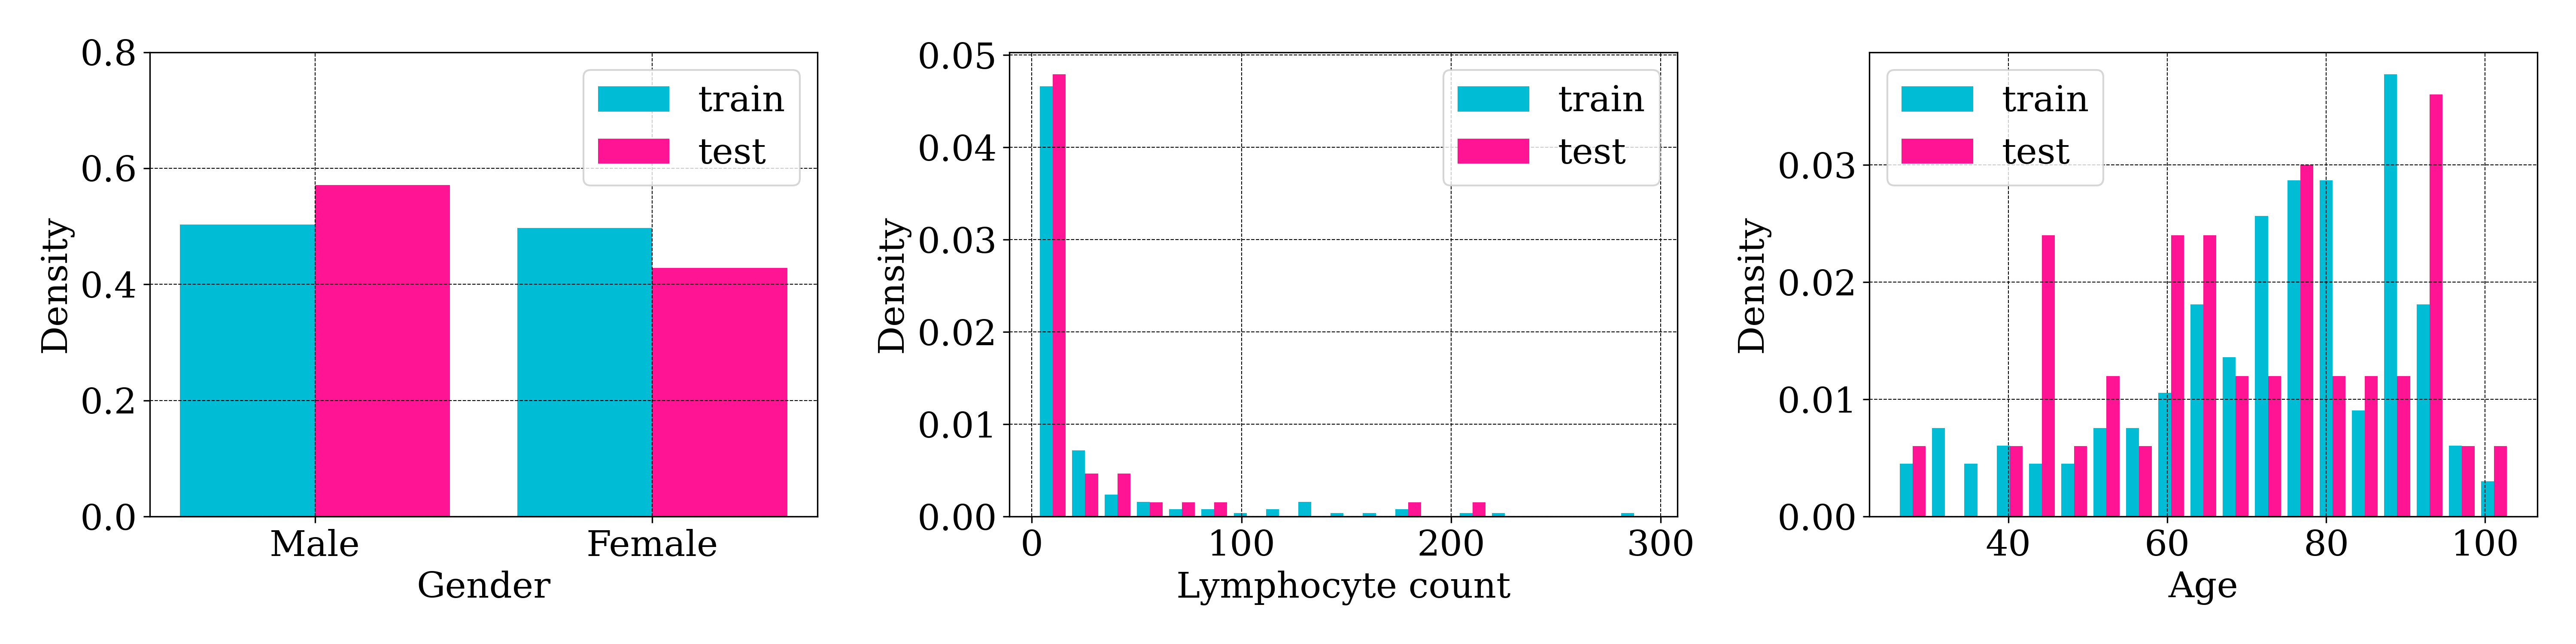
\includegraphics[width=0.9\textwidth]{figures/train_test_histograms.png}
    \caption{Histograms of the training and test datasets.}
    \label{fig:train_test_histograms}
\end{figure}

On figure \ref{fig:positive_negative_histograms}, we observe the distribution of the positive and negative classes in the training dataset. While gender does not seem to be a good predictor of the negative (reactive) or positive (malignant) class, a high lymphocyte count seems to be a good indicator of malignant lymphocytosis. The malignant nature is also more prevalent in older patients.

\begin{figure}[h!]
    \centering
    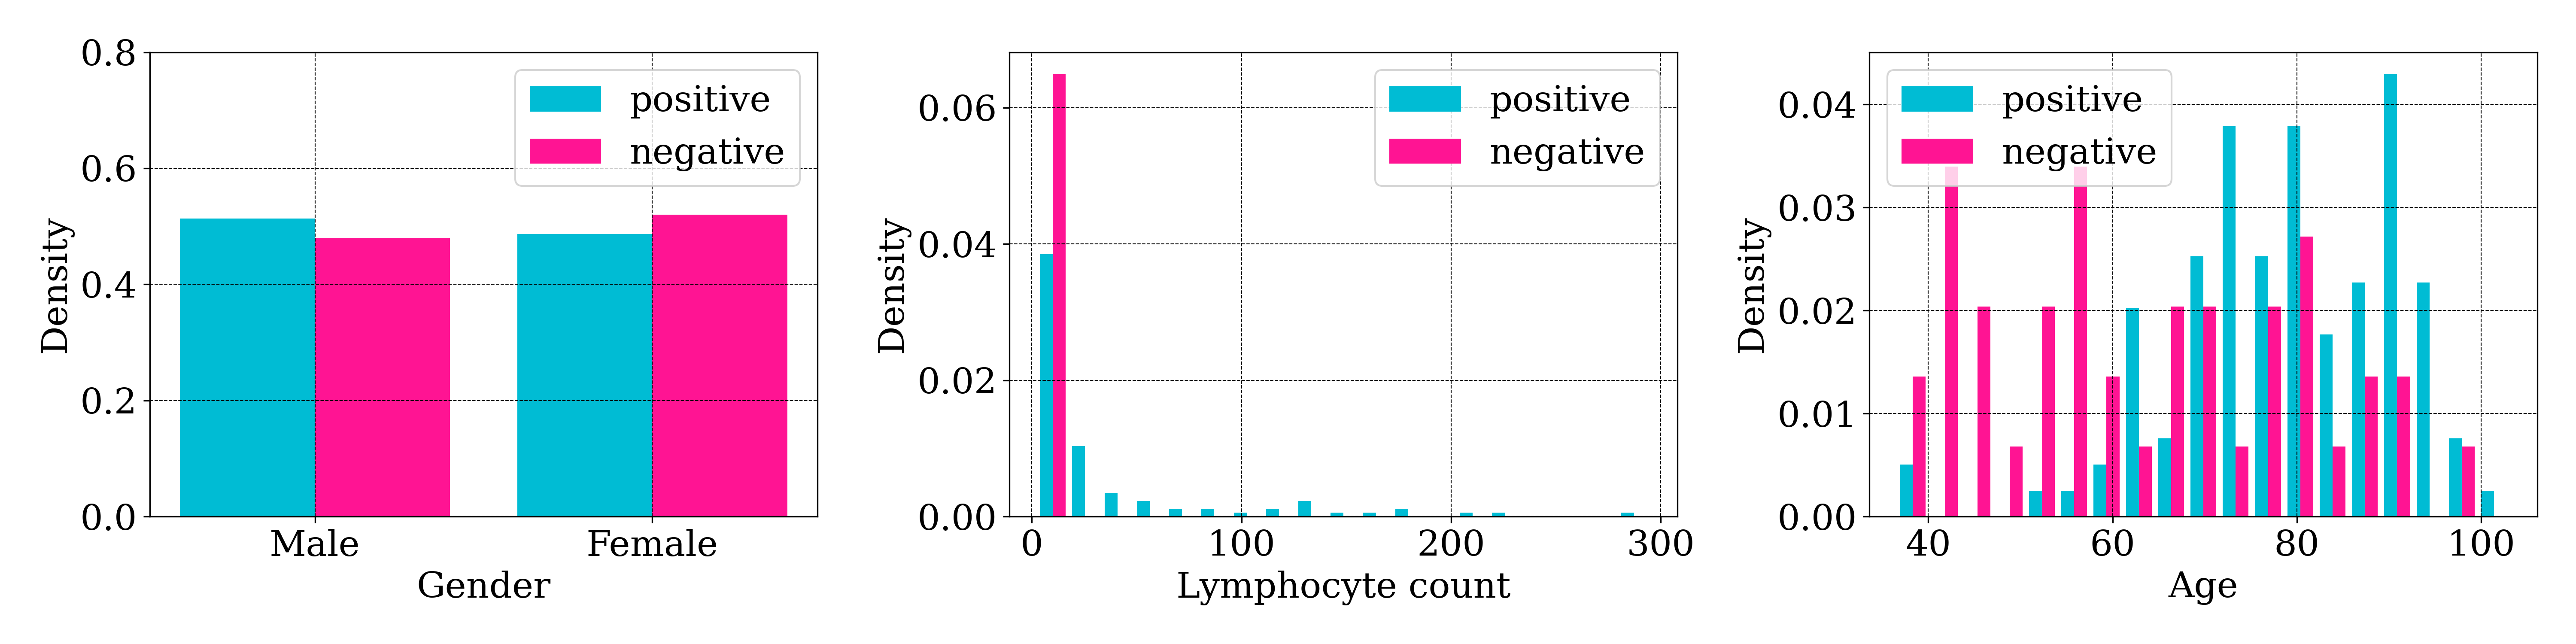
\includegraphics[width=0.9\textwidth]{figures/positive_negative_histograms.png}
    \caption{Histograms of the positive and negative classes in the training dataset.}
    \label{fig:positive_negative_histograms}
\end{figure}

The imbalance between the positive and negative classes ([TODO HOW MUCH]) justifies the use of a stratified split of the training dataset between training and validation sets, i.e. we split the dataset in a way that the proportion of positive and negative classes is the same in the training and validation sets. We also normalize the lymphocyte count and age features to be between 0 and 1.

\section{Model tuning and comparison}
\label{sec:evaluation}

\section{Conclusions}
\label{sec:conclusion}

\newpage
\bibliography{bibliography}

\end{document}